\chapter{Results}


\begin{center}
    \textit{This chapter presents the outcomes of the project, including the functionality and performance of the developed application. It highlights the achieved results in relation to the project goals and requirements.}
\end{center}

\section{Machine Learning Model}

As described in Section~\ref{subsec:model-testing}, the model was evaluated using 100 games. Table~\ref{tab:accuracy-total} presents the overall move detection accuracy, both in total and broken down by piece type and color. The model achieved an overall accuracy of 90.6\%, successfully detecting 936 out of 1033 moves. Pawns had the highest detection rates, with over 98\% accuracy for both colors. In contrast, the model struggled particularly with black rooks with only 23.8\% accuracy.

% \newpage

\begin{table}[htbp]
\centering
\caption{Move detection accuracy in total}
\label{tab:accuracy-total}
\begin{tabular}{lccc}
\toprule
\textbf{Category} & \textbf{OTB Moves} & \textbf{Successful Moves} & \textbf{Accuracy (\%)} \\
\midrule
\textbf{White Pieces} & & & \\
\hspace{1em}Pawn  & 244 & 242 & 99.2\% \\
\hspace{1em}Knight & 128 & 117 & 91.4\% \\
\hspace{1em}Bishop & 74  & 54  & 73.0\% \\
\hspace{1em}Rook   & 29  & 25  & 86.2\% \\
\hspace{1em}Queen  & 42  & 40  & 95.2\% \\
\hspace{1em}King   & 16  & 8   & 50.0\% \\
\midrule
\textbf{Black Pieces} & & & \\
\hspace{1em}Pawn  & 247 & 243 & 98.4\% \\
\hspace{1em}Knight & 78  & 75  & 96.2\% \\
\hspace{1em}Bishop & 65  & 47  & 72.3\% \\
\hspace{1em}Rook   & 21  & 5   & 23.8\% \\
\hspace{1em}Queen  & 84  & 76  & 90.5\% \\
\hspace{1em}King   & 5   & 4   & 80.0\% \\
\midrule
\textbf{Total} & 1033 & 936 & 90.6\% \\
\bottomrule
\end{tabular}
\end{table}


Table~\ref{tab:board-type-accuracy} compares the success rates between the two physical board types used during testing. The wooden board slightly outperformed the plastic board, with a 91.2\% success rate compared to 89.9\%. This marginal difference may indicate a slightly more stable detection environment on the wooden surface. \\


\begin{table}[htbp]
\centering
\caption{Summary of Total Moves and Success Rate by Board Type}
\label{tab:board-type-accuracy}
\begin{tabular}{lccc}
\toprule
\textbf{Board Type} & \textbf{Total Moves} & \textbf{Total Successful Moves} & \textbf{Success Rate (\%)} \\
\midrule
Plastic & 475 & 427 & 89.9\% \\
Wooden  & 558 & 509 & 91.2\% \\
\bottomrule
\end{tabular}
\end{table}


% \newpage

Figure~\ref{fig:move-failures} shows the number of failed games (i.e., games where detection failed) grouped by the move number at which failure occurred. Bars are color-coded by board type. The majority of failures occurred within the first five moves, particularly at moves 2, 4, and 5. This trend suggests that the early game presents the greatest challenge for detection, potentially due to rapid development or ambiguity in piece positions. Notably, failures after move 9 were rare. \\


\begin{figure}[htbp]
\centering
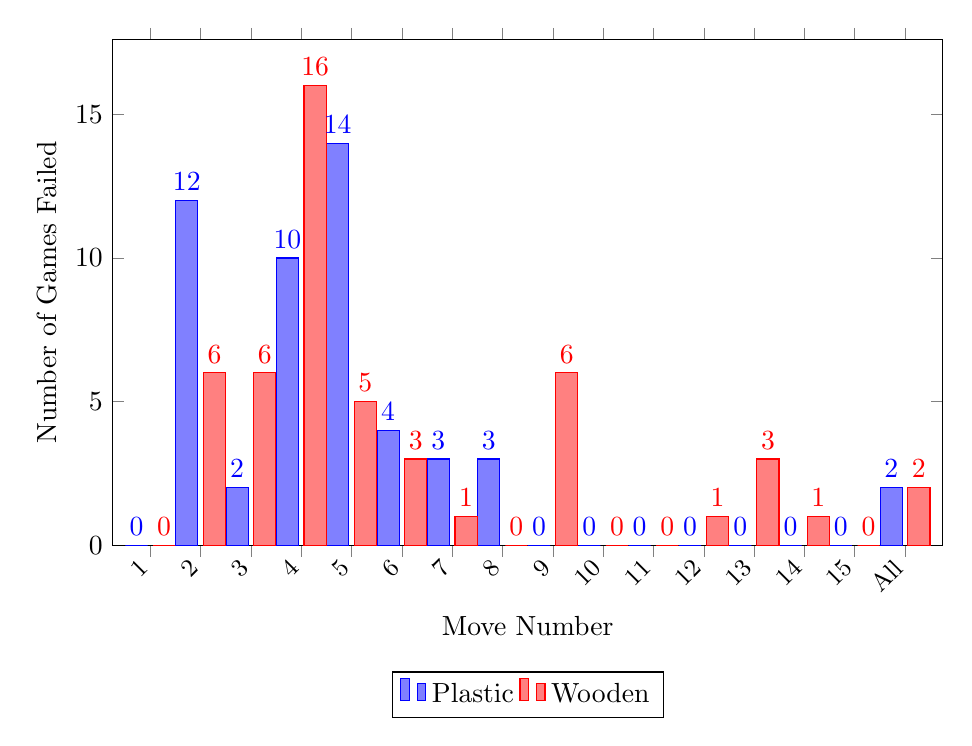
\begin{tikzpicture}
\begin{axis}[
    ybar,
    bar width=8pt,
    width=\textwidth,
    height=8cm,
    enlarge x limits=0.05,
    ymin=0,
    ylabel={Number of Games Failed},
    xlabel={Move Number},
    xtick={1,...,15,All},
    xticklabels={1,2,3,4,5,6,7,8,9,10,11,12,13,14,15,All},
    x tick label style={rotate=45, anchor=east},
    legend style={at={(0.5,-0.25)}, anchor=north, legend columns=-1},
    nodes near coords,
    symbolic x coords={1,2,3,4,5,6,7,8,9,10,11,12,13,14,15,All},
    xticklabel style={font=\small},
]
\addplot+[style={fill=blue!50}] coordinates {
    (1,0) (2,12) (3,2) (4,10) (5,14) (6,4) (7,3) (8,3) (9,0)
    (10,0) (11,0) (12,0) (13,0) (14,0) (15,0) (All,2)
};
\addplot+[style={fill=red!50}] coordinates {
    (1,0) (2,6) (3,6) (4,16) (5,5) (6,3) (7,1) (8,0) (9,6)
    (10,0) (11,0) (12,1) (13,3) (14,1) (15,0) (All,2)
};
\legend{Plastic, Wooden}
\end{axis}
\end{tikzpicture}
\caption{Number of failed games per move number across plastic and wooden boards.}
\label{fig:move-failures}
\end{figure}


Table~\ref{tab:different-errors} categorizes the types of detection failures for each board type. The majority of failures were due to a complete lack of detection within the allotted time window. Incorrect detections (the model detecting a move but interpreting it wrongly) were less frequent but more common on the wooden board, accounting for 8 out of 48 failures, compared to just 1 on the plastic board.  \\

\begin{table}[htbp]
\centering
\caption{Frequencies of Different Detection Errors}
\label{tab:different-errors}
\begin{tabular}{lccc}
\toprule
\textbf{Board Type} & \textbf{Total Failures} & \textbf{No Detection} & \textbf{Incorrect Detection} \\
\midrule
Plastic & 48 & 47 & 1 \\
Wooden & 48 & 40 & 8 \\
\midrule
\textbf{Total} & 96 & 87 & 9 \\
\bottomrule
\end{tabular}
\end{table}

For a detailed breakdown of the chess games, including the sequences of moves, failure points, and detection statistics for each board type, see Appendix FILL IN.

% \newpage

\section{Overview of Delivered Product}
The delivered product refers to the final version of the application submitted at the conclusion of this Bachelor’s thesis. The application was developed at the request of the product owner and based on the requirements provided. The initial description served as a general concept rather than a detailed specification, which meant that decisions regarding design, architecture, and technology were left to the development team. Throughout the development process, ideas and design choices were discussed with the product owner and approved during regular meetings. \\

The application was developed as an open-source project with the intention that the code can be reused, maintained, and extended by others. All components are built using open and freely available technologies, ensuring that the system can be installed on local hardware without the need for licensed software or cloud-based services. This aligns with the requirement that all processing should be performed locally, using common hardware such as a webcam connected to a local machine running either Windows or Ubuntu. \\

The project follows clear coding standards and development best practices, making the code easy to understand and modify. All functionality is well documented, enabling future developers to build upon the existing solution. For example, to support new chess variants, integrate additional hardware, or improve the recognition models. To support future development and accessibility, the source code is published in a public Git repository without restrictions on reuse or adaptation. \\

The application itself is a local, camera-based system for digitalizing over-the-board chess games in real time. It detects piece movements on a physical chessboard using image recognition and converts the game into a \gls{pgn} file, which can be viewed or analyzed digitally. The system operates entirely on local hardware, with a front-end interface that allows users to follow games live and a back-end that manages board recognition and game logic. The application is designed to be low-cost, open-source, and easy to maintain, with extensibility in mind for future features.

\section{Functional Results}
The application consists of three main components: machine learning, WebSocket communication, and the frontend interface. The backend handles image recognition and game logic, using a machine learning model to detect board states. It communicates with the frontend through a WebSocket connection. The front-end is responsible for presenting this information to the user in real time. The cameras is connected with a \acrshort{usb}-hub, where multiple cameras can be attached to the same computer. 

\subsection{API}
To enable real-time updates and improve the responsiveness of the frontend interface, the application uses a WebSocket connection between the backend and the frontend. This method was suggested by the product owner and was also approved by the supervisor. This communication channel is used for transmitting move data as it is detected by the board recognition system. Unlike traditional \gls{http} requests, which operate on a request-response basis, WebSocket allows for continuous, two-way communication between the server and the client as outlined in Subsubsection \ref{subsubsec:websocket} in Section \ref{chp:theory}. \\

Once the application initiates a connection, the WebSocket remains open throughout the session. As new moves are identified on the physical board, the backend sends the corresponding move data as messages through the WebSocket. These messages are then received by the frontend, which updates the displayed move list and board state in real-time. This provides a seamless viewing experience for users following live games. \\

The WebSocket server also handles specific command messages. For example, when the server sends a message labeled \texttt{RESET}, the frontend clears the current move list typically indicating the start of a new game. The \texttt{RESET} command also resets the backend system, alloweing for a new tournament round to begin. A message labeled \texttt{INVALID} is used to signal an unrecognized or incorrect move and does not trigger any frontend changes. All other messages are assumed to be valid algebraic notation representing chess moves and are appended to the game history displayed to the user. \\

The WebSocket functionality is encapsulated in a custom React hook on the frontend, which manages the connection lifecycle and state updates. This abstraction simplifies integration into the user interface and ensures that resources are properly cleaned up when the component is unmounted. Overall, the use of WebSocket communication is a key component in delivering a responsive and live experience, particularly for tournaments and public displays where move-by-move tracking is essential.

\subsection{Frontend}
\label{subsec:results-frontend}
The front-end of the application serves as the user interface. It includes a control panel for tournament organizers and a web application for spectators. The application's main responsibility is to visualize the chessboard and display ongoing moves. The front-end communicates with the back-end via WebSocket to ensure real-time updates and interactivity. \\

The control panel is a standalone administrative interface used exclusively by tournament organizers to configure and manage the tournament setup. Accessible only from the host computer, it allows the organizer to select the number of camera inputs, initiate the tournament, and reset boards between rounds, as shown in Figure~\ref{fig:control-panel}. This interface ensures the secure and centralized management of tournament operations. \\

\begin{figure}[h!] \centering 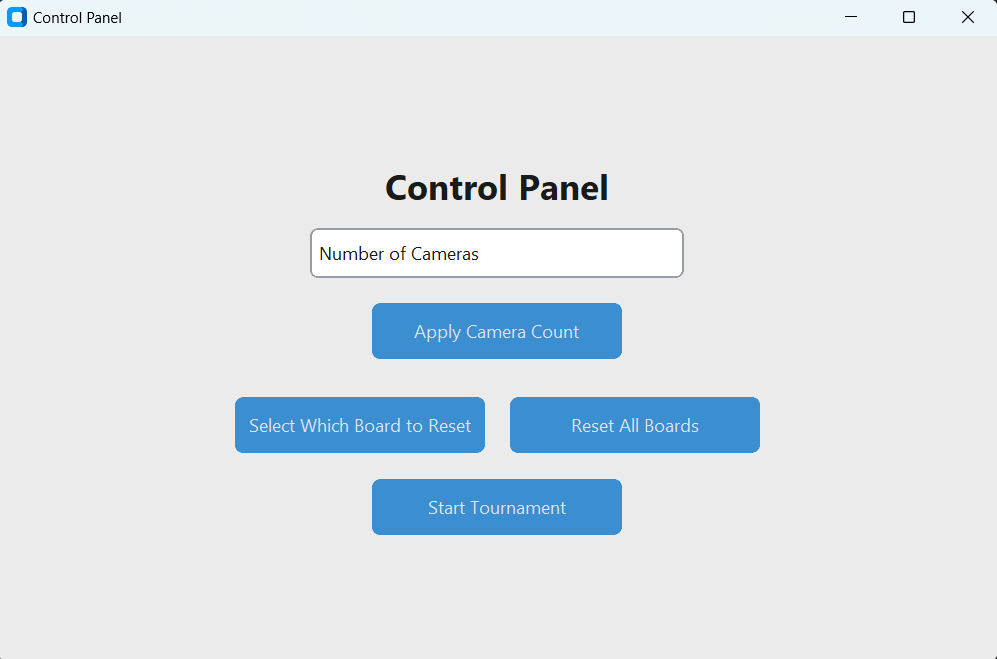
\includegraphics[width=0.75\linewidth]{figures/results/frontend/control-panel/control-panel.png} \caption[Control panel for tournament organizers]{The control panel used by the tournament organizers.}\label{fig:control-panel} \end{figure}

Once the application is launched, the accompanying web application becomes accessible to spectators. It is designed to allow viewers to follow the tournament in real time across a range of devices. Built as a responsive interface, it adapts to both desktop and mobile screens to ensure accessibility and usability. Spectators can navigate between views, observe live games, and explore additional information about the system. \\

One of the main pages in the web application is the Tournament View, which presents an overview of all ongoing games. Each entry shows the board number, the players' names and ratings, and a link to follow the game live, as shown in Figure~\ref{fig:tournament-view-mocked}. The content is updated continuously, providing spectators with a live snapshot of the tournament's progress. \\

\begin{figure}[h!] \centering \fbox{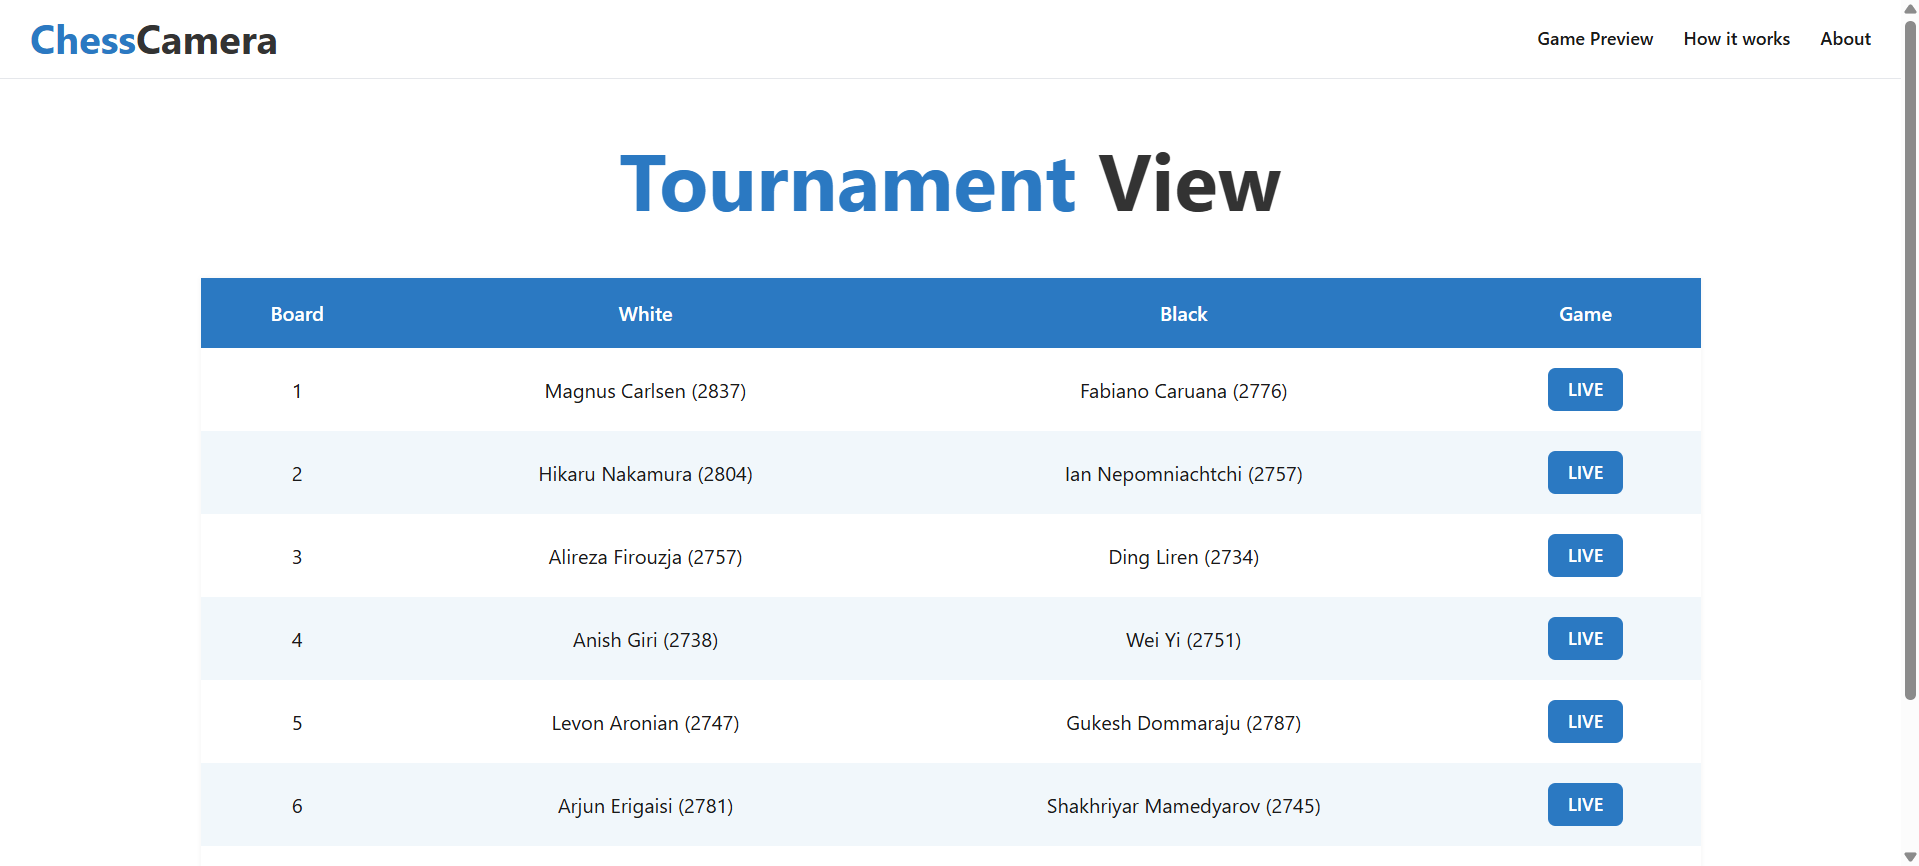
\includegraphics[width=0.75\linewidth]{figures/results/frontend/tournament-view/mocked.png}}\caption[Display of tournament]{A mocked demonstration of a tournament display.}\label{fig:tournament-view-mocked} \end{figure}

Another page is the Board View, which focuses on a single game in greater detail. This view includes a digital chessboard, a list of moves played, a live camera feed, and a visual evaluation bar, as shown in Figure~\ref{fig:board-view-mocked}. The elements update in real time, creating an engaging and intuitive experience for users following a particular match. \\

\begin{figure}[h!] \centering \fbox{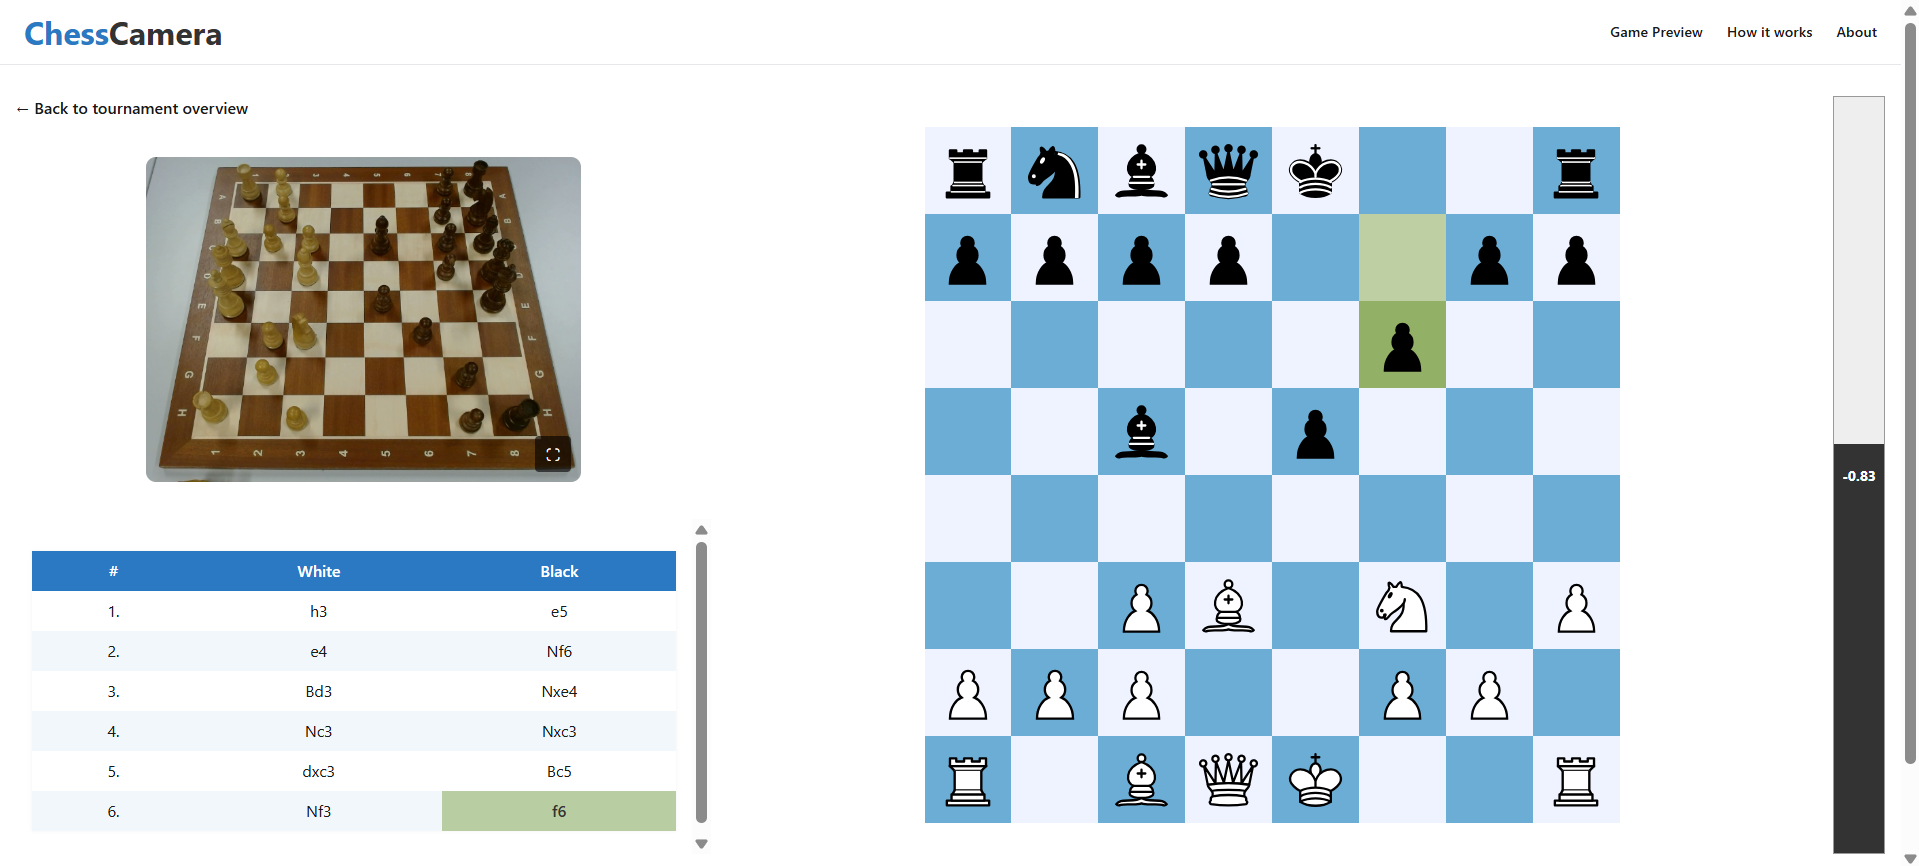
\includegraphics[width=0.75\linewidth]{figures/results/frontend/board-view/desktop.png}}\caption[Display of a board]{A mocked demonstration of an active game}\label{fig:board-view-mocked} \end{figure}

In addition, the web application features a Game Preview page that displays simplified mini-boards for multiple games. This view enables users to quickly glance through active games and select one to view in detail, as shown in Figure~\ref{fig:game-preview}. It offers a compact and efficient way to stay updated on several games at once. \\

\begin{figure}[h!] \centering \fbox{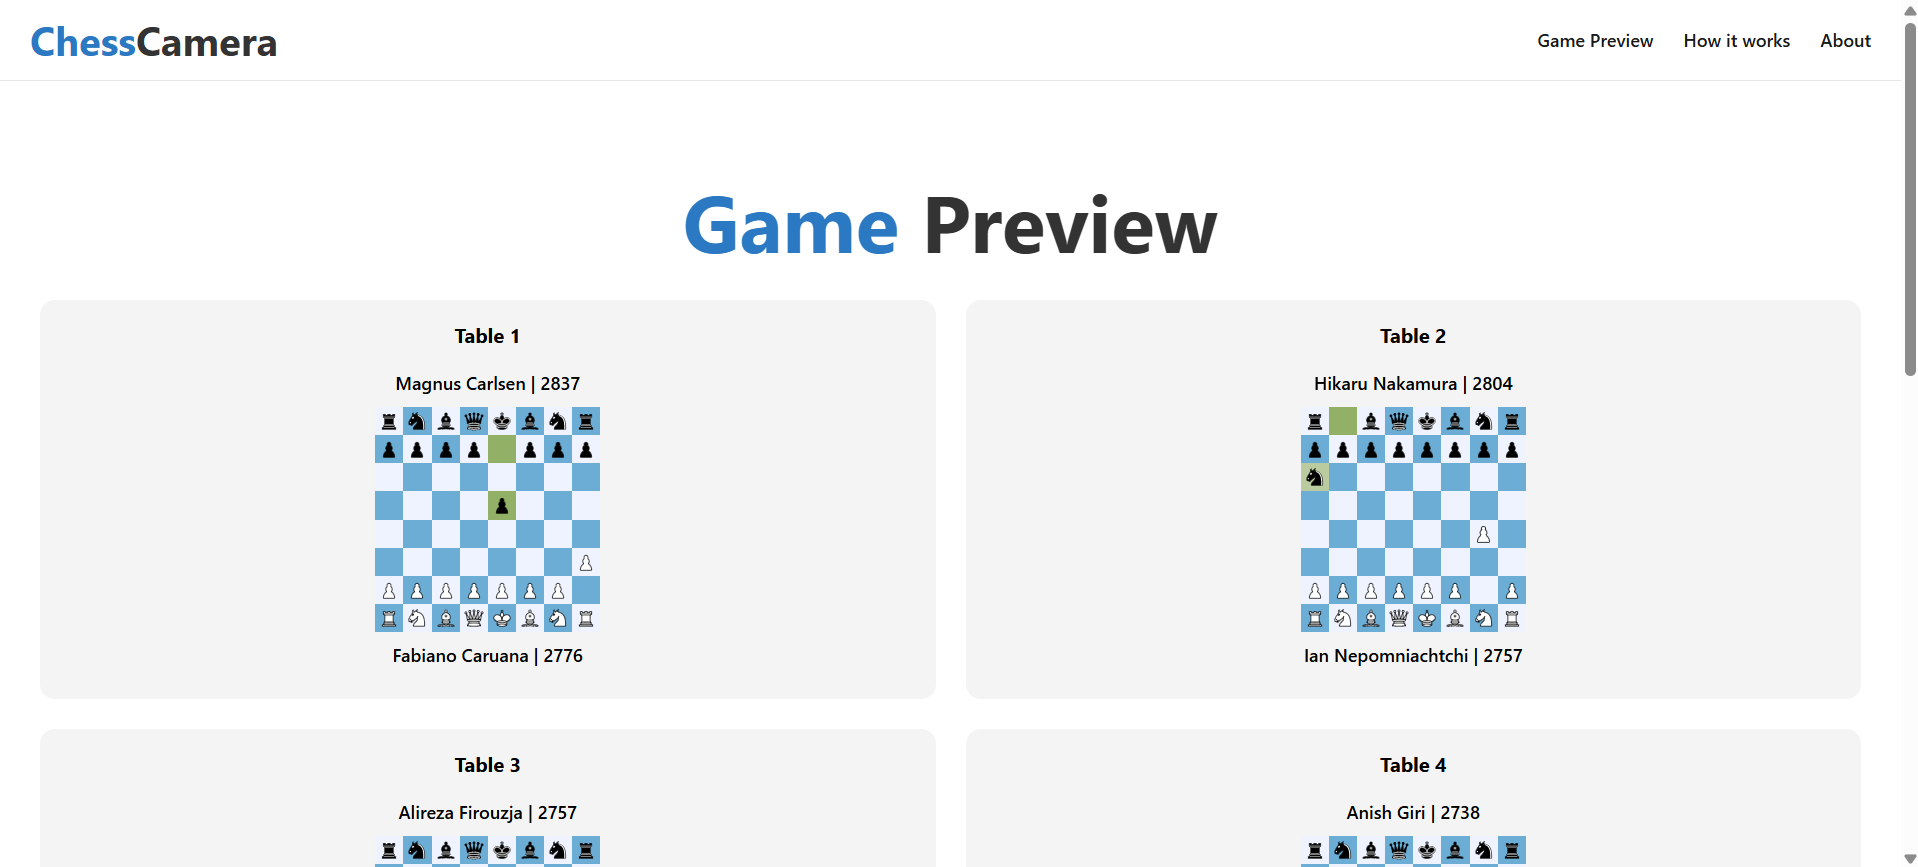
\includegraphics[width=0.75\linewidth]{figures/results/frontend/game-preview/desktop.png}}\caption[Preview of active games]{A mocked demonstration of a game preview page.}\label{fig:game-preview} \end{figure}

The user also has the option of downloading the \gls{pgn} file for a selected game. On the board view page, a dedicated button allows the user to download the \gls{pgn} file corresponding to the game currently displayed. When this button is clicked, the file is saved locally on the user's computer, as shown in Figure~\ref{fig:download-pgn}. \\

\begin{figure}[h!] \centering \fbox{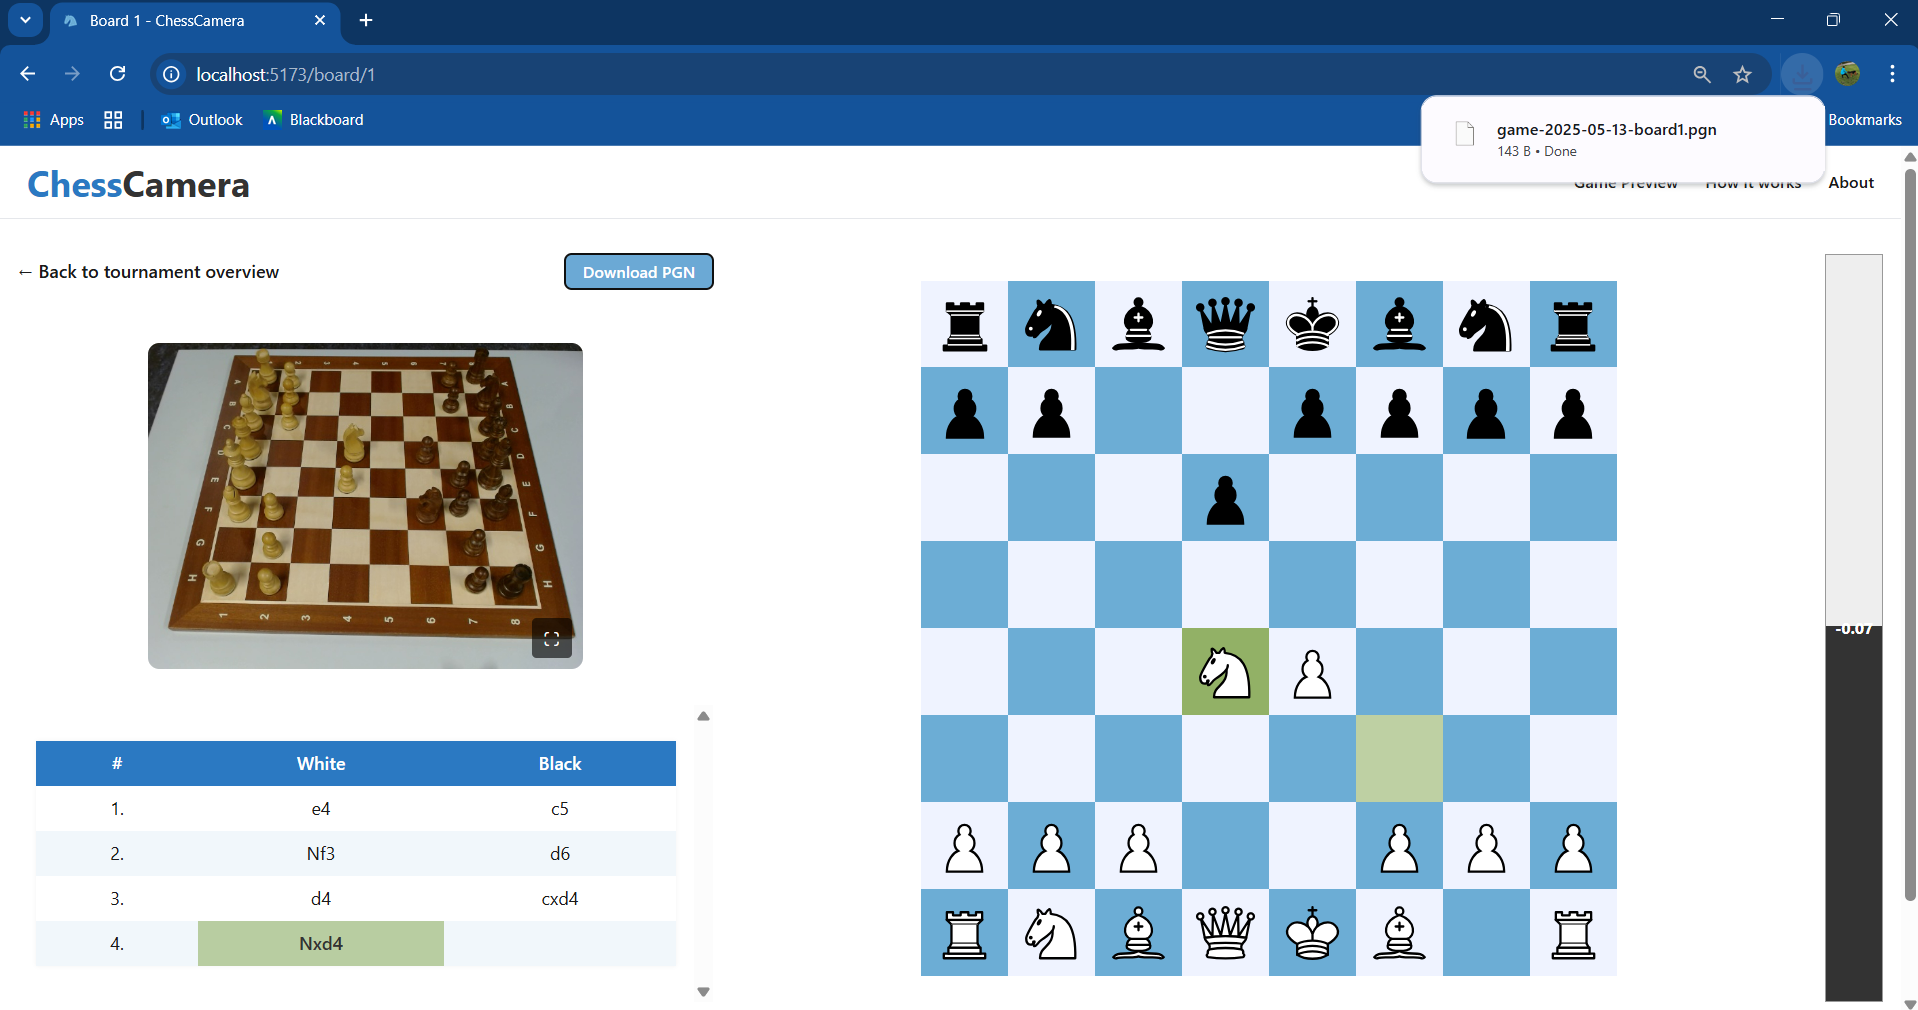
\includegraphics[width=0.75\linewidth]{figures/results/frontend/download-pgn/download-pgn.png}}\caption[Preview of downloading a PGN file]{A demonstration of downloading a PGN file to a specific game}\label{fig:download-pgn} \end{figure}

The downloaded file includes a header with key information such as the tournament name, date, and player names, followed by the recorded list of moves. An example of this file opened in a code editor is shown in Figure~\ref{fig:downloaded-pgn}. In this case, the game is still ongoing, so not all moves have been logged, and the result is marked as "in progress," indicating that the \gls{pgn} file is incomplete. \\

\begin{figure}[h!] \centering \fbox{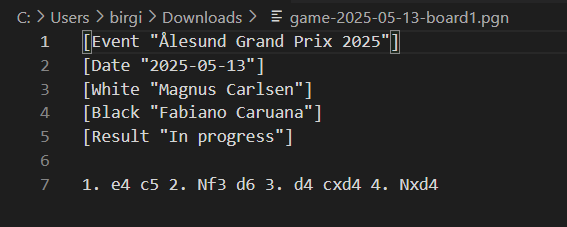
\includegraphics[width=0.75\linewidth]{figures/results/frontend/download-pgn/downloaded-pgn.png}}\caption[The downloaded PGN file]{The downloaded PGN file to a specific game, opened in a code editor}\label{fig:downloaded-pgn} \end{figure}

\section{Project Management}
\label{sec:results-project-management}
Although the project was initially structured according to the Scrum framework, its practical execution became more Scrum-inspired due to the absence of a dedicated Scrum Master and certain deviations from the full methodology. Each sprint began with a planning session in which tasks were selected from the product backlog based on priority and available team capacity. Sprint reviews were conducted at the end of each sprint to assess completed work and record outcomes. In addition, sprint retrospectives were held and documented, including reflections on workload distribution, communication challenges, and opportunities for process improvement. \\

Meeting routines were adapted according to team availability and project needs. Internal meetings were held as needed rather than on a fixed schedule, with most collaboration taking place informally during shared office hours. Nevertheless, short stand-up meetings were prioritized on a daily basis to maintain effective communication and ensure alignment. Biweekly meetings with the supervisor were consistently maintained, functioning as checkpoints for academic progress and clarification of requirements. Meetings with the product owner were arranged approximately once or twice per month and typically focused on feature validation, feedback, and adjustments. \\

GitHub was used consistently throughout the project for both task management and version control. Issues were linked to corresponding branches and categorized by type (e.g., feature, enhancement, documentation). All code changes were submitted via pull requests, and no changes were pushed directly to the main branch. Peer review was strictly enforced as part of the workflow, with every pull request reviewed by at least one team member before merging. \\

Tasks were assigned to individual team members and tracked using GitHub Issues. Issues were labeled and moved through the workflow stages: \textit{No Status}, \textit{To Do}, \textit{In Progress}, and \textit{Done}. This workflow was followed consistently for larger development tasks. However, some minor items, particularly quick fixes and small adjustments, were occasionally completed outside of the issue board during periods of intensive development, resulting in slightly reduced traceability for those changes.\\

\subsection{Architecture Overview}
\label{subsec:diagrams}

To provide a comprehensive understanding of the system architecture and interaction flow, several \gls{uml} diagrams were created. These diagrams model different aspects of the live chess game digitization system, from component interactions and activity flow to user roles and use cases.

\subsubsection*{Sequence Diagram}
\label{subsubsec:sequence-diagram}

The sequence diagram, shown in Figure \ref{fig:sequence}, illustrates the chronological flow of interactions between the system components and external actors. It begins with the Admin initiating the game recording by setting up the camera, which captures and streams the board state to a local processing unit. This unit continuously detects and validates moves, updating the user interface accordingly. Users, from remote devices, can spectate the game in real time or save it as a \gls{pgn} file. The diagram emphasizes the communication between hardware (camera and local machine) and the \gls{ui}, highlighting how physical chess games are digitized and broadcasted.

\newpage

\begin{figure}[h!]
    \centering
    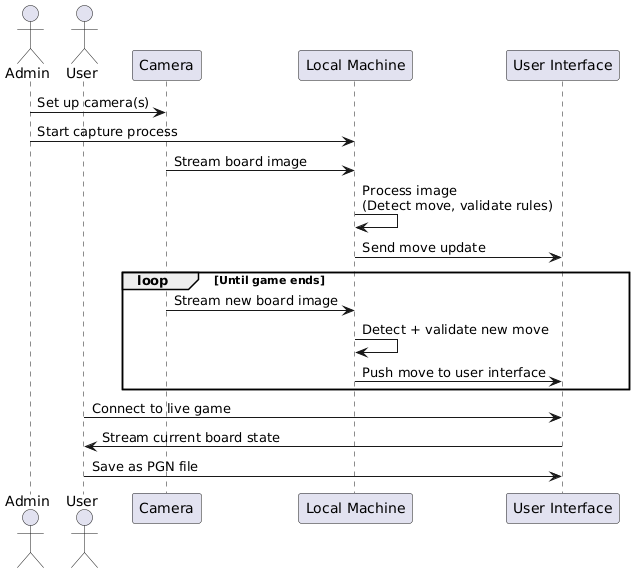
\includegraphics[width=0.75\linewidth]{figures/methods/uml/sequence.png}
    \caption[Sequence Diagram]{Sequence Diagram}
    \label{fig:sequence}
\end{figure}

\subsubsection*{Use-Case Diagram}
\label{subsubsec:use-case-diagram}

The use-case diagram, shown in Figure \ref{fig:use-case}, identifies the system’s main actors and the primary functionalities they interact with. Admins are responsible for hardware setup and initiating the game recording process. The system autonomously handles move detection, validation, and \gls{ui} updates. Users, on the other hand, access the game remotely to spectate or download \gls{pgn} files. This diagram provides a clear overview of who interacts with the system and what capabilities are exposed, forming the basis for understanding system requirements and user expectations.

\begin{figure}[h!]
    \centering
    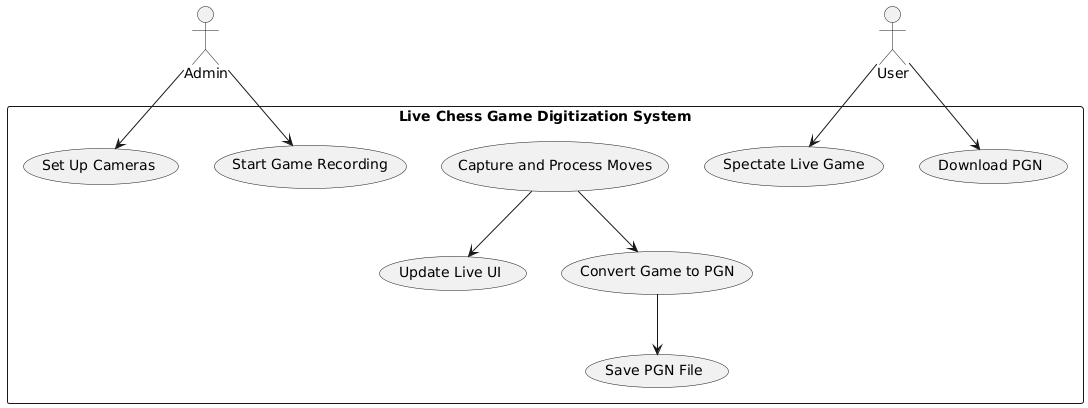
\includegraphics[width=0.75\linewidth]{figures/methods/uml/use-case.png}
    \caption{Use-Case Diagram}
    \label{fig:use-case}
\end{figure}

\begin{figure}[h!]
    \subsubsection*{Activity Diagram}
    \label{subsubsec:activity-diagram}
    
    \centering
    \begin{minipage}[t]{0.5\textwidth}
        \vspace{0pt}
        The activity diagram, shown in Figure \ref{fig:activity}, provides a high-level overview of the operational workflow during a chess game session. It models the continuous loop of capturing board states, detecting and validating moves, and updating the game state until the game ends. If a move is invalid, the system flags it but does not terminate the session. Once the game concludes, it is converted into a standard \gls{pgn} format. This diagram emphasizes the logical flow and decision-making process, reflecting the system’s role in automating and maintaining the integrity of live digitization.
    \end{minipage}
    \hfill
    \begin{minipage}[t]{0.45\textwidth}
        \vspace{0pt}
        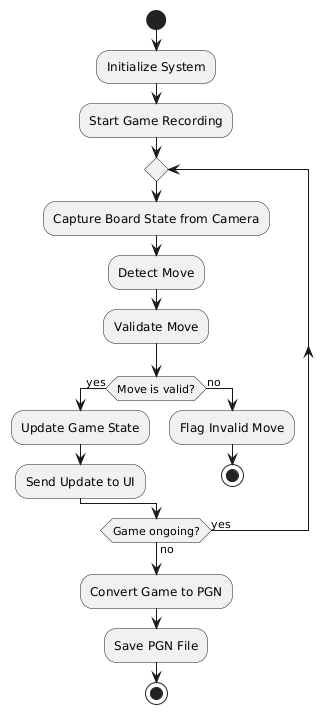
\includegraphics[width=\linewidth]{figures/methods/uml/activity-2.png}
        \caption[Activity Diagram]{Activity Diagram}
        \label{fig:activity}
    \end{minipage}
\end{figure}

\section{Testing and Quality Assurance}
\textit{Summary of testing performed (unit tests, integration tests, manual testing). Test coverage results or bugs discovered/fixed. If relevant, include tables or graphs showing test results or reliability.}

\subsection{Manual Testing}



\subsection{Wireframe Testing}
\label{subsec:results-wireframe}
The testes revealed how these users experienced the structure of the wireframes. The wireframe's overall experience averages on 4,63. The Tournament View averaged on 4,75. The Board View averaged 4,38. 

\begin{figure}[htbp]
\centering
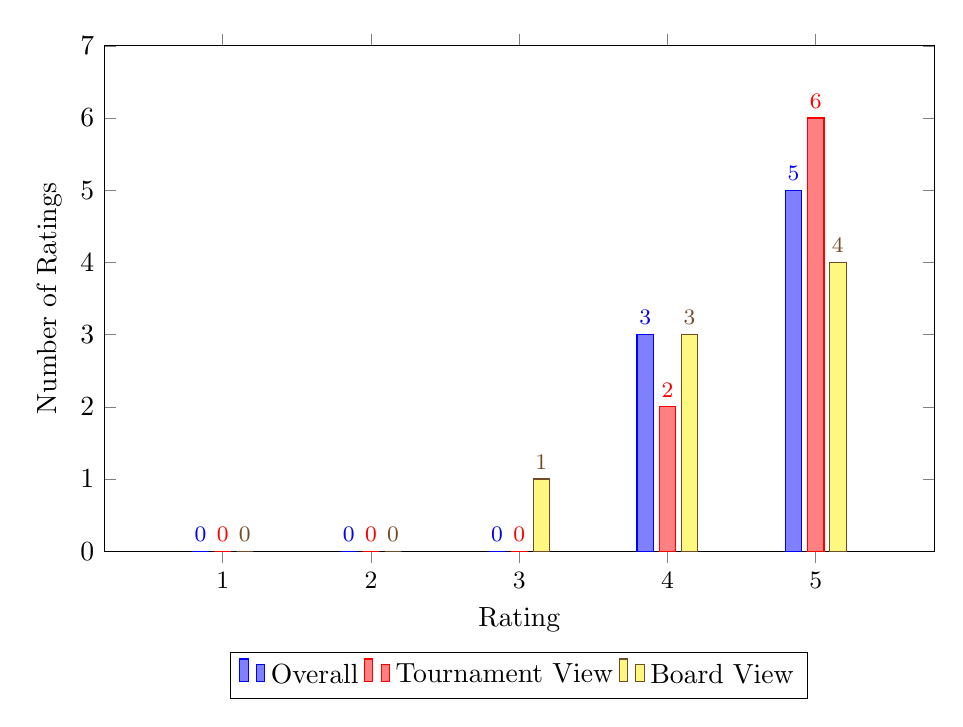
\begin{tikzpicture}
\begin{axis}[
    ybar,
    bar width=6pt,
    width=\textwidth,
    height=8cm,
    enlarge x limits=0.2,
    ymin=0,
    ymax=7,
    ylabel={Number of Ratings},
    xlabel={Rating},
    symbolic x coords={1,2,3,4,5},
    xtick=data,
    x tick label style={rotate=0, anchor=north, font=\small},
    legend style={
        at={(0.5,-0.2)},
        anchor=north,
        legend columns=3
    },
    nodes near coords,
    nodes near coords style={font=\footnotesize},
    every node near coord/.append style={
        /pgf/number format/.cd,
        fixed,
        precision=0,
        /tikz/ifthenelse/.code={
            \ifnum\pgfplotspointmeta=0
                \pgfkeys{/pgfplots/disable node}
            \fi
        }
    }
]
\addplot+[style={fill=blue!50}] coordinates {
    (1,0) (2,0) (3,0) (4,3) (5,5)
};
\addplot+[style={fill=red!50}] coordinates {
    (1,0) (2,0) (3,0) (4,2) (5,6)
};
\addplot+[style={fill=yellow!50}] coordinates {
    (1,0) (2,0) (3,1) (4,3) (5,4)
};
\legend{Overall,Tournament View,Board View}
\end{axis}
\end{tikzpicture}
\caption{Distrubution of ratings}
\label{fig:move-failures}
\end{figure}



\subsection{Color Palette}
\label{subsec:results-color-palette}
Voting revealed a mix of preferences: some participants favored the light mode from palette \#08 and the dark mode from palette \#07, while others selected the board design from palette \#05 or the move-highlighting style from palette \#14. \\

Rather than selecting a single predefined palette, the final color scheme was assembled by combining the most highly rated elements across the top-voted variations, yielding a more tailored, user-informed visual design. Figure \ref{fig:color-palette-results} shows the distribution of votes across all tested palettes; the full set of prototypes appears in Appendix \ref{app:color-palettes}.

\begin{figure}[htbp]
\centering
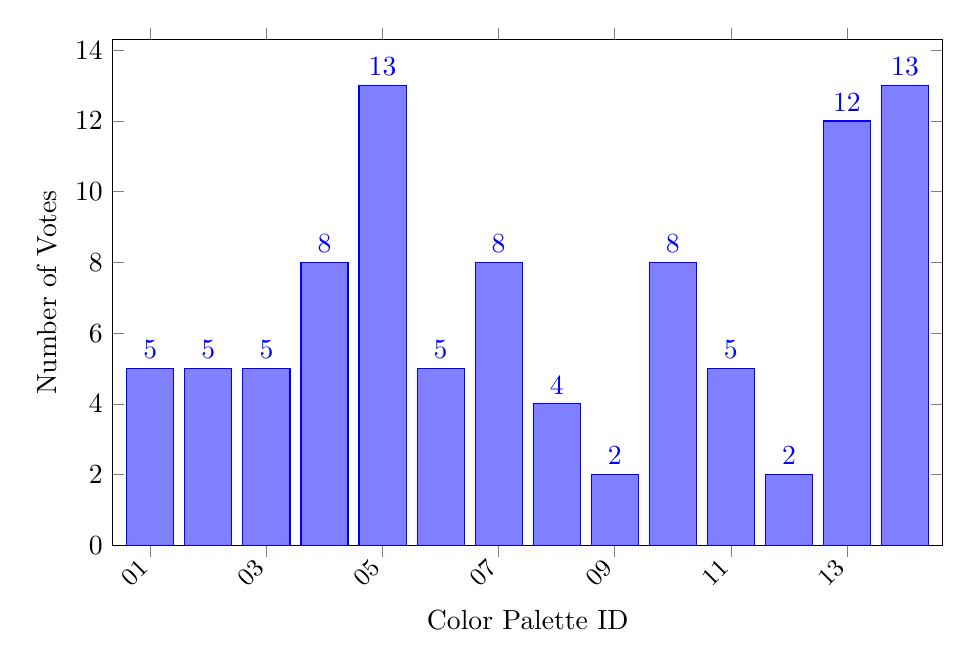
\begin{tikzpicture}
\begin{axis}[
    ybar,
    bar width=17pt,
    width=\textwidth,
    height=8cm,
    enlarge x limits=0.05,
    ymin=0,
    ylabel={Number of Votes},
    xlabel={Color Palette ID},
    xticklabels={01,02,03,04,05,06,07,08,09,10,11,12,13,14},
    x tick label style={rotate=45, anchor=east},
    nodes near coords,
    symbolic x coords={01,02,03,04,05,06,07,08,09,10,11,12,13,14},
    xticklabel style={font=\small},
]
\addplot+[style={fill=blue!50}] coordinates {
    (01, 5) (02, 5) (03, 5) (04, 8) (05, 13) (06, 5) (07, 8) (08, 4) (09, 2) (10, 8) (11, 5) (12, 2) (13, 12) (14, 13)
};
\end{axis}
\end{tikzpicture}
\caption{Distribution of Votes Across Different Color Palettes}
\label{fig:color-palette-results}
\end{figure}